\documentclass[10pt]{article}
\usepackage[CHN]{iscv}
\usepackage{capt-of}
\usepackage{hologo}
\bibliographystyle{ieeetr}

\setlength{\parindent}{4ex}

\title{电车难题之思————浅谈后果主义解决伦理困境之优越性}
\author{浙江大学 \and 土水交 \and 徐子安}

\begin{document}

% \twocolumn[{%
% \maketitle
% \begin{center}
%     \centering
%     \includegraphics[width=.9\linewidth,height=4cm]{example-image-golden}
%     \captionof{figure}{Teaser Image}
% \end{center}%
% }]
\maketitle

\abstract
摘要写在这里。摘要应简明地概括文章的主要内容。

\keywords 后果主义, 伦理冲突, 利己主义

\section{引言}
      “哲学来源于生活”。
   
      哲学应当是生活中自然演化和孕育出的。通常我们在决定和评判一件事情的时候,我们并不知道自己所抱持的观点与什么哲学家相似————但往往它们真的曾被人提出过。
     
    作者并没有太多哲学领域的专业知识,只能说站在哲学的门口,正仰望着这片神圣的城池,还并没有踏入半分。

  全文手写(打),除了引用没有复制粘贴半分。我写这篇(如果能够称得上的话)论文,不只是为了作一篇课程的成果,也是给自己多年思考的一个小结。

\section{电车难题:“电车”为何成为“难题”}
    这是一个大家耳熟能详的思想游戏。

      在讨论伦理学问题的时候,“电车难题”往往是用来启发学生思考和讨论的良好范例。作者在此便以“电车难题”为例,阐释我所思考之“后果主义”,与康德所秉持的道德,与大家所秉持的道德,究竟有何差异和优劣。
      
      电车难题的传统情景如下:
      

\emph{
 一辆失控的列车在铁轨上行驶。在列车正行进的轨道上,有五个人被绑起来,无法动弹。列车将要碾压过他们。您正站在车站内,离改变列车轨道的操纵杆很近。如果您拉动此杆,则列车将切换到备用轨道上。但是,您会注意到备用轨道上只有一个人被绑着。您有两种选择:
 }
    \begin{itemize}
        \item \emph{1. 什么也不做,让列车按照正常路线碾压过这五个人。}
        \item \emph{2. 拉下操纵杆,改变为备用轨道,使列车压过备用轨道上的另一个人。}
        \end{itemize}

   我们先来解读这个场景的含义。在此之前,我们先做一个约定:在理解像“电车难题”这样的思想游戏的时候,我们不能无意义地避开这个思想游戏的核心。例如,在电车难题的情境下,他需要你在生命之间做出选择,你就不应当给出“通过不牺牲生命的方式”解决问题的策略。这不是一个现实问题,不需要完美的答案,它只需要你对这个矛盾核心本身的思考。
   
   它预设了一个十分极端的生命选择场景。也就是,你需要在“五条生命”和“一条生命”之间做出选择。其他的限制条件诸如“列车”“轨道”之类的要素可以忽略,你也不需要知道为什么六个活人会被奇奇怪怪地绑在铁轨上。你只需要知道,现在裁决者是你,你需要做出你的选择。
   
    
 \begin{figure}[h]
\centering
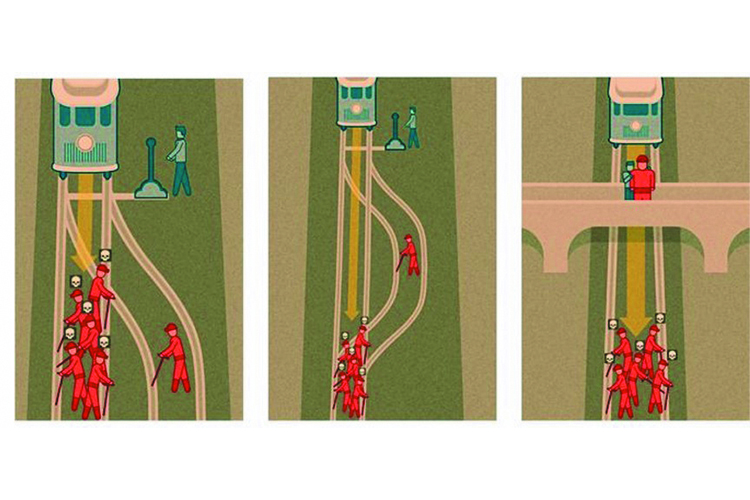
\includegraphics[width=.9\linewidth]{figs/电车难题示意图.jpeg}
\caption{电车难题} 
\label{fig:example}
\end{figure}
 
   
    \subsection{经典道德(康德义务论)对电车难题的回答}
    在课堂讨论中,坚定地抱持义务论观点的同学往往难以做出选择————在这样的理论中,生命应当是绝对的、至高的。任何情况下,直接或者间接导致生命消亡的行为,都是应当受到谴责的。同样你也不能将五条生命和一条生命进行对比————无穷与无穷,没有哪一个更大。
    这样的思考矛盾可以这样表述:
    1. (基本预设)生命是无价的。任何直接或间接导致(无辜的)生命消亡的行为,都是错误的、值得谴责的。
    2. (情景难题)我们的行为无论如何都会导致(无辜)生命的死亡。
    3. (结论)我们的行为无论如何都是错误的。

   \subsection{我们为何不能解决电车难题}
   为什么我们无法解决电车难题?\par
    电车难题的核心是在拷问我们对生命的看法。你在你的道德体系中,将生命置于一个怎样的地位。生命是否能用数量来简单衡量?当生命遭到破坏的时候,我们如何行动? 
    \par
    电车难题反映出的其实是经典道德义务论在一些极端场景下,自身原本具有的矛盾性。\par
    这套道德伦理本身并不保证自洽。“生命无价”的观点,“生命不可被侵犯”的戒律,原本是基于人们的审美、基于人们既有的直觉的道德观念,从诞生之初便不以“解决问题”为根本使命,不保证在任何情况下互不冲突,更不保证在任何情况下都能给出人们“给如何做”的指导。\par
    我觉得“电车难题”是传统道德伦理不完备性的一个小小体现。在更广的维度上,在更多的哲学思想游戏中,甚至是在一些社会问题上,我们可以看到更多这样困境的发生。那些受到热议的、无法被轻易决定对错的实例,往往是因为类似的原因:当双方都有对有错,双方都不应当被牺牲,可是矛盾发生了,我们如何处置这种情形?

    我无法忍受这种矛盾和冲突。出于个人的角度来说,我希望自己奉行的思考方式坚定而稳固,时时刻刻为我提供有力的决策参考。这就是为什么我更偏爱以后果来决定价值的这样一套行为方法论————我的“后果主义”。

\section{何为后果主义:以后果定义价值}
在解释我所说的后果主义的基本原则之前,先来谈谈我对它的一些理解。
    
    “电车难题”本身是道德伦理学中,用来展现功利主义对行为义务论的优势的一个情景。可在这样的情境下,我强调的是后果主义的优越性。我来解释一下其中的原因。
     
    我认为的后果主义,只规定“对‘后果’的无条件追求”这一条戒律。至于什么样的后果是好的,什么样的后果会被定义为是不尽人意的,不是后果主义的规定范围。我更愿意将它看作是更多伦理学规范的一个关节————当你将“实现最大多数人的利益”作为最优的后果的时候,那它就是功利主义;当你将这个主体限制在自己、限制在极少的个体的时候,那它就是利己主义。
          
    我觉得利己主义和功利主义,在这样的情形下都能给出坚定而明确的回答。为什么?因为对后果的明确指向和坚定追求。因此,我将这一部分单独提出来,作为一个单独的关节用来讨论。
    
    \subsection{后果主义的基本观点}
      
    后果主义者抱持以下观点:
      
     \begin{itemize}
    \item \emph{ 一件事情的正确性应当由它的后果来决定,而不是其他任何与后果无关的元素。}
    \item  \emph{ 后果主义者在任何时候都应当坚定地追求,在现有的条件下所能获得的最好的后果。}
    \end{itemize}
       
   这两条规定,看上去十分明确易懂。但事实上其中蕴含了非常多的信息。
     
   首先,是对一系列价值的颠覆。第一条规则其实否定了很多我们习以为常的价值定义。我们在做出个人决策的时候,常常不仅将后果作为唯一的参考因素————诸如道德观点,诸如喜恶,等等等等。 但后果主义的这一条规定消解了所有这样的思考元素————除了“后果”占据最高的地位,除了后果追求的对象(也许是个人或者他人的利益)具有先验的价值,其他任何元素应当平权,应当平行地纳入考量。
     
   就像是在电车难题的情境下,也许我们最终会做出某样选择,但往往在考虑的过程中,将“生命”本身也作为十分重要的因素纳入考量,带有十分沉重的负罪感或者内疚感进行决策。可是对于后果主义者而言,一样行为,不会因为“符合传统道德”,或者是“因为拯救了生命”而成为正确的行为,而只能因为“对我达成后果有利”而间接地具有正确性。或者说,后果主义者不承认“传统道德”的突出地位,尤其是在“后果”面前的突出地位。
      
   因此,后果主义者在对电车难题做出回答的时候,应当是毫不犹豫、毫无负担地————如果我是功利主义者,我应当也必须选择大多数人的利益,无论五个人在哪条轨道上,我必须尽一切可能去拯救他们;如果我是利己主义者,我也许会选择袖手旁观,因为这样会造成对我最少的舆论谴责。但无论如何,行为都是坚定地、自洽的,在他们自己的道德逻辑中,自己已经完满地解决了这个问题。

   接下来,我们将通过一些例子,来深入地理解后果主义的以上观点和一些衍生观点。
    
   \subsection{后果主义不关心“同一”}
     
     后果主义强调对第一条原则的坚定贯彻。不仅仅在行为的维度上,甚至在认知的维度上。我们对第一条基本观点作如下引理:
     
    \begin{itemize}
    \item \emph{1. 当两件事情造成的影响相同,我们就认为它们一样。}
    
    \item \emp{2. 如果事情不产生任何后果,我们就认为它们不存在。无论这件事情是否真的存在。}
    \end{itemize}
    
    暂借认识论中另一个十分有趣的思想游戏————忒修斯之船,来略作说明。忒休斯之船背景如下:
    
    \emph{
    这是一则非常古老的思想实验,也称为认知“悖论”。忒修斯是传说中的雅典国王。式修斯号是以他的名字命名的一艘船,它标志着战争胜利的荣耀。在克里特岛归还时,国王与雅典年轻人搭乘了这艘有30个桨的船,后被雅典人作为纪念。
     }
     \par
     \emph{
  随着时间的流逝,式修斯号船的木板逐渐腐朽,而只要哪块木板老旧腐烂,雅典人就会立刻换上新的木板来替代。终于有一天,该船的每根木板都被换了一遍。
}
\par
\emph{
  古希腊哲学家对此发问:“这艘船还是原来的那艘忒修斯号船吗?如果是,但它已经没有最初的任何一根木头了;如果不是,那它是从什么时候开始就不是了?”
}
\par
\emph{
   哲学家托马斯·霍布斯将这个问题弄得更加复杂:如果有人将换下来的老旧配件收集起来,再做成一艘船,与那艘由新配件组成的“式修斯号”相比,哪一艘才是真正的忒修斯号呢?
}
\par
    
    在课堂对这个问题进行讨论的时候,大家对这个问题的理解仅仅局限在“是否同一”,以及“为何同一”。在大家没有抱持相同基础观点的情况下,其实讨论者之间并没有办法彻底理解和接受对方的观点。后果主义便提供了一个这样的基础,并且简单而明确地解决了这个问题。
      
    后果主义不关心同一。因为“同一”本身不造成任何影响。我们认为无限接近和同一是一样的,或者更明确一点,直接从理论体系中删掉“同一”这个东西。\par
    如果我是乘船者,我只需要关心这两艘船是否具有相同的航行性能,如果在这个层面上一样,那就是一样的;如果我是考古学家,我只需要关心这两艘船是否都有我需要的历史遗留,既然没有,那显然不一样;如果我是想把它做成旅游景点的投资人,我只需要考虑换了木板是否会对景区的火爆程度造成影响。不论在哪种情形下,我认为只要仿照到了极致,那就是一样的。\par
    这不是一种退避,对问题视而不见,并不是忽略了或者避开了问题本身。后果主义给出了相当后果主义的回答。

    在这个问题中,后果主义不同于其它思考方式的地方在于,它选择舍弃这种理想的“绝对”。这种“舍弃”,对无必要无意义概念的舍弃,对“本质”本身的否定,使得它在解决许多伦理困境下展现出强有力的优越性。我认为这是一种创造性的策略,它是后果主义解决问题优越性的重要来源之一。

    “沙子问题”也同样可以得到回答:\par
  \emph{
  一顿沙子堆在一起,是一顿沙子。现在你从里面拿掉一粒,它还是一堆沙子。你不断地拿走一粒一粒,请问在被拿完之前,什么时候它不是一堆沙子了?  
  }   
  \par
    对于这样的问题,后果主义同样保持相同的回答:当这个概念对我们理解沙子无意义的时候,就可以将它删去。“一堆沙子”是一个概念,指向某个数量范围内的沙子。它能够存在的前提,就是说话者和倾听者不关心什么时候它不是一堆沙子。
       
    在另外一些场景下,我们可以选择其他恰当的描述方式:无论什么时候,沙子的集合都必定具有确定的质量、确定的数目,会造成确定的后果。当我需要知道它的重量,我就去称重;当我需要知道它的数目,我就费劲去数。但在任何情况下,它“是不是一堆沙子”都没有任何影响。买沙子的人会关心这里有多少吨,但绝不会关心着是不是一堆沙子。
   
    后果主义者抱持这样的观点:概念只是为了我们更好地描述这个世界。当概念本身成为了解世界和描述世界的阻碍时,我们就应该放弃它们。后果主义否定“概念”本身的价值。反对将价值与“概念”本身直接绑定,而选择在需要的时候,用解构的、用精确的方式来描述事物。沙子什么时候成为一堆不重要,多重、多少粒才重要;就像行为是否符合道德不重要,是否能获取想要的后果才重要。

 \subsection {后果主义:“有限决策”原则}
    
    这样的后果主义显然地会引起很多质疑。
    
    在功利主义的受到的批评之中,较为严重的一个问题是,你如何计算最大的幸福,如何计算最大的利益。在遇到复杂的情境的时候,我们必须要做到最好,意味着必须全知全能。而这是不可能的。
    
    我的后果主义第二条基本观点,对此问题做出了修正的回答————“有限决策”原则:我只做我认知中最好的决策;混沌便是相等,未知便是平权。
    计算机解决问题有一个策略,叫近似最优解。当你没有办法在整个过程中得到最优解的时候,没有办法找到代价最小的那条路,那就在走到一个地方的时候,做出当下最好的选择。也许“当下最好”走完的路径代价是“最好路径”的百分之一百二十、百分之一百五十,但你花费的算力可能是它的千分之一甚至是万分之一。

    在我受限的视角中,我不在乎如何决策是事实上的最好。在我的视角中,根据我现在掌握的信息判断,这样的后果是最好的,那我就这么办。事实上究竟是不是,我不关心。
    例如,我需要为天下大多数人谋福祉,我现在可以选择医生或者老师这两个职业。当然它们都是前途远大的职业,都能给他人带来光明和希望。我不知道哪一个会带来更多的福祉,我可以做更多的事情,这两个选项的价值对我来说是混沌的,那我就随便选。因为在未知的问题上投入思考是低效的————你永远无法预测世界会如何变化。有这个工夫,你不如思考如何把自己选择的职业干好。

    我想,“没有达到最优”不应当成为批评理论的原因。如果想达到“最优”,你应该去问科学,而不是哲学。没有哪一种哲学体系可以帮助你在任何情形下做出最优的选择————后果主义在努力地这样做,它在试图排除掉一切干扰性的因素,排除掉一切阻挡在科学决策面前的障碍,我相信,相比其他的行为范式,后果主义做得更好。
    
\section{后果主义:强大包容性}
    
\section{后果主义观察小记:自我反思}


    (如果这不适合加入论文里,那我会把它删掉。)
    
    我要开始胡说八道了。
    
\subsection{“追求走向反面”的迷思}

我一直在疑惑一个问题。
   
   世界上有没有什么东西,是必须纯粹,不能用后果来度量的?
  我所找到的结果,最可能接近的结果,是爱和人性。也许它们必须要被无条件地相信,才能展现出自己的价值。当“爱”不再被无条件地接受,而必须与“满足孤寂的需要”和“向往其中的美好”这样的动机挂钩,它可能就成为了永远追求不到的东西。
  后果主义的解构太过于强大,我越来越无法接受相反的逻辑:我愿意和你待在一起,不是因为需要什么,不是因为要你给我什么,它毫无缘由、毫不在乎影响,仅仅是存在,所以有理由,如此而已。
   
  当你坚定地秉持后果主义,将一个人的福祉作为最高的要素,通过适当的调控和配置,或许你能拥有最好的人缘,拥有最好的财富和能力,但你一定摆脱不了寂寞。后果主义者会需要一种热烈的激情,需要那个目标一直引诱你向前冲刺,当他停下来看这个世界的时候,只能看见无底的空虚和寂寞。
   
  我一开始给自己制定的后果,究竟是否正确?我选择解构一切,不相信一切,追问一切,究竟是否正确?在某一个瞬间,我想换一种思考方式,我不需要最大化的结果,甚至不需要计算到的最大的幸福和快乐,我只想单纯地相信些什么,也许这样就已经足够幸福了。
  
\subsection{后果主义的出身背景}
  这思想有非常浓重的个人色彩。
  
 我被训练成为一个优秀的掠夺机器。出身于平凡得不能再平凡的家庭,父母终日为生活琐事所忙碌。我从来没有被教育过“寄予”,我无法理解“寄予”和纯粹的利他,无法理解纯粹的美好,我理解世界的运行本质为“交换”。
  
  我习惯性地将“获得”作为最大的目的。后果主义天生默认“获得”为最大的义务,没有给出具体而平等的论证。后果主义天生是一种工具,我反复强调它是一种思维范式,而不是一个具有指导性的世界观。从电车难题那里开始,我选择祛魅生命的价值,选择祛魅道德,最终究竟丢弃了什么?我不知道,我也很惶恐。

  在我看来,后果主义的思维方式更像是一种狭隘的世界观的产物————被生活本身的烟火气所限制,被欲望和贪婪限制,尤其是它们被美化为“积极和进取”之后————像是阶级跃迁或者是生活不易的牺牲品。

  我从小被认为具有成熟的思想。我不喜欢玩,不喜欢很多别人喜欢的东西,而会希望自己比别人做得好一点、看得远一点。毫无理由地。

  这是一种一无所有的害怕。对将来的不确定的害怕,对自己生活不稳定的害怕,对人生本质是否虚无的害怕。(所以我一直在强调这种思想范式必须帮助我做出决策)这是一种全阶级甚至全社会都共有的情绪,驱使着我们不断去掠夺,去获得更多的东西。我只是这股洪流中的小小一者,后果主义不过是诸多精致利己者的一个托辞而已。

  我在这里遇到了一些我曾经无法想象的思想。也许并不是所有人都害怕失去,并不是所有人都在如此强烈地寻求安全感。 总有人有权利或者是有想法,去诗意地栖居。说实话这使我十分震惊。
  
  我觉得,后果主义不应该是我的希望。至少在被生活的重压击倒之前,在社会污浊侵扰之前,我想明白什么是真正的幸福和快乐。

% \begin{itemize}
%     \item 论文: 最多 4 页
%     \item 技术报告: 最多 2 页
%     \item 新闻稿: 1 页
% \end{itemize}

% 页数统计包含文章所有图表,但不包含参考文献。如果有补充材料,包括图片、详细分析、视频等,可以发表在论坛上。
% 若投稿被接收,作者将会受邀在研讨会上讲解自己的工作。

% 所有投稿需要使用 B5  (17.6 cm $\times$ 24 cm) 纸,文章内容应在纸张中心的 {14 cm $\times$ 20 cm} 范围内,即页面上下边距为 2cm,左右边距为 1.8cm.
% 投稿的论文和技术报告需要双栏排版。

% \subsection{图表}
% 文章图表需要居中放在每一栏中,并按其出现的顺序编号。每一个图、表下方应包含标题和编号 (示例见图~\ref{fig:example}或表~\ref{tab:example})。
% 注意图表中的文字不要过大或过小。
% 对于需要横跨双栏的图表,可以使用 \texttt{figure*} 或 \texttt{table*}环境, 跨栏图表应使用\texttt{[t]} 或 \texttt{[b]} 选项将其置于页面顶端或底端。

% \begin{figure}[h]
% \centering
% 
\includegraphics[width=.5\linewidth]{figs/fig1.pdf}
% \caption{示例图片} 
% \label{fig:example}
% \end{figure}

% \begin{table}[h]
% \centering\begin{tabular}{ccc}
% \toprule
% Net & top1 & top5 \\
% \midrule
% ResNet & 7\% & 5\% \\
% VGG & 10\% & 7\% \\
% ShuffleNet & 15\% & 10\% \\
% \bottomrule
% \end{tabular}
% \caption{示例表格}
% \label{tab:example}
% \end{table}

% \subsection{公式}
% 文中独立出现的文字应居中排版,并按其出现的顺序编号。编号应向右对齐,并由圆括号包围。使用 \LaTeX 排版时会自动生成公式编号。
% 在引用公式时,使用 \verb|\eqref{eq:label}| 产生正确的引用格式,如式~\eqref{eq:example}。
% \begin{equation}
% \label{eq:example}
% 	    PA + A'P - PBR^{-1}B'P + Q  =  0
% \end{equation}

% \chapter{生成 PDF 文件}
% 最终文献以 PDF 为标准格式。使用 \LaTeX{} 排版,并用 \hologo{XeLaTeX} 编译则会自动生成符合要求的 PDF 文件。建议使用 Overleaf 处理 \LaTeX{} 文件。

% \chapter{参考文献}
% 参考文献列表应与引用顺序一致。文中引用文献应使用方括号形式,例如文献~\cite{ref01}和文献~\cite{ref01,ref02}。

\acknowledgements
致谢。


\end{document}
